\documentclass{beamer}[10pt, usepdftitle=false, handout]

\beamertemplatenavigationsymbolsempty

\usepackage[T1]{fontenc}
\usepackage[]{algorithm2e}
\usepackage{multimedia}
\usepackage{gensymb}
\usepackage{textcomp}

%\usepackage[font=small,labelfont=bf]{caption} 

\usetheme{Boadilla}

\title{Basic of Computer Networks 3}
\author[]{Paul Blondel}
\institute[]{CNAM}
\date[]{March 1st, 2019}

\usepackage[style=british]{csquotes}


\def\signed #1{{\leavevmode\unskip\nobreak\hfil\penalty50\hskip1em
  \hbox{}\nobreak\hfill #1%
  \parfillskip=0pt \finalhyphendemerits=0 \endgraf}}

\newsavebox\mybox
\newenvironment{aquote}[1]
  {\savebox\mybox{#1}\begin{quote}\openautoquote\hspace*{-.7ex}}
  {\unskip\closeautoquote\vspace*{1mm}\signed{\usebox\mybox}\end{quote}}


\setbeamertemplate{headline}
{
  \leavevmode%
  \hbox{%
  \begin{beamercolorbox}[wd=1.0\paperwidth,ht=2.25ex,dp=1ex,center]{author in head/foot}%
    \usebeamerfont{author in head/foot}\insertsubsection
  \end{beamercolorbox}}%
  \vskip0pt%
}


\setbeamertemplate{footline}
{
  \leavevmode%
  \hbox{%
  \begin{beamercolorbox}[wd=.5\paperwidth,ht=2.25ex,dp=1ex,center]{author in head/foot}%
    \usebeamerfont{author in head/foot}\insertsection
  \end{beamercolorbox}%
  \begin{beamercolorbox}[wd=.5\paperwidth,ht=2.25ex,dp=1ex,center]{title in head/foot}%
    \usebeamerfont{title in head/foot} \inserttitle \hspace*{2em}  \insertframenumber{} / \inserttotalframenumber\hspace*{2ex} 
  \end{beamercolorbox}}%
  \vskip0pt%
}

\AtBeginSection[]
{
   \begin{frame}
    \tableofcontents[ 
    currentsection] 
   \end{frame}
}

\begin{document}
	{
	\setbeamertemplate{footline}{
  	\leavevmode%
  	\hbox{%
  	\begin{beamercolorbox}[wd=.5\paperwidth,ht=2.25ex,dp=1ex,center]{author in head/foot}%
  	\end{beamercolorbox}%
  	\begin{beamercolorbox}[wd=.5\paperwidth,ht=2.25ex,dp=1ex,center]{title in head/foot}%
  	\end{beamercolorbox}}%
  	\vskip0pt%	
	} 
	\begin{frame}
	\titlepage
	\end{frame}

	\begin{frame}
	
	\begin{aquote}{Tim-Bernes Lee - Creator of the WEB}
I think, in general, it's clear that most bad things come from misunderstanding, and communication is generally the way to resolve misunderstandings — and the Web's a form of communications — so it generally should be good.
	\end{aquote}	
	
	\end{frame}


	\begin{frame}
		\tableofcontents
	\end{frame}
	}

	\addtocounter{framenumber}{-3}

	\section{Traffic concentration}	
	\subsection{What is it?}

    \begin{frame}[label=(first)]
	
	But what if now there are more than two computers?
	\vspace*{1em}	
	
	The resources must be shared so that information can be shared.
	\vspace*{1em}	
	
	Resources can be shared if the sum of the activities ($\theta$) of several users is smaller than or equal to 1 (1=resources fully occupied).
	
	\vspace*{1em}	
	
	$\sum_{i=1}^{i=n}\theta_{i} \leq 1$
	\vspace*{1em}	
	
	This is called: traffic concentration. 
	
	\end{frame}	 
	 
	\begin{frame}
	
	\begin{center}	
	\begin{figure}
		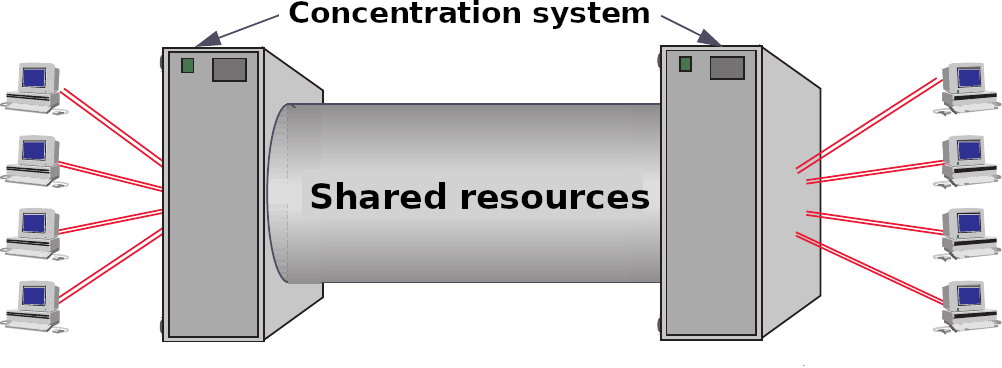
\includegraphics[scale=0.4]{images/3-1.png} 
     	%\vspace*{-0.5em}
		%\caption{Floating gate transistor cell}
	\end{figure}	
	\end{center}
	
	We can distinguish three different concentration approaches:
	\vspace*{1em}
	
	\begin{enumerate}
	\item{Concentrators: allowing 1 -> N and N -> 1 links}
	\item{Multiplexers: allowing 1 -> 1 links}
	\item{Networks: allowing 1 -> 1 to N links (or even M -> 1 to N links)}	
	\end{enumerate}			
	\vspace*{1em}	
	
	\begin{center}	
	\begin{figure}
		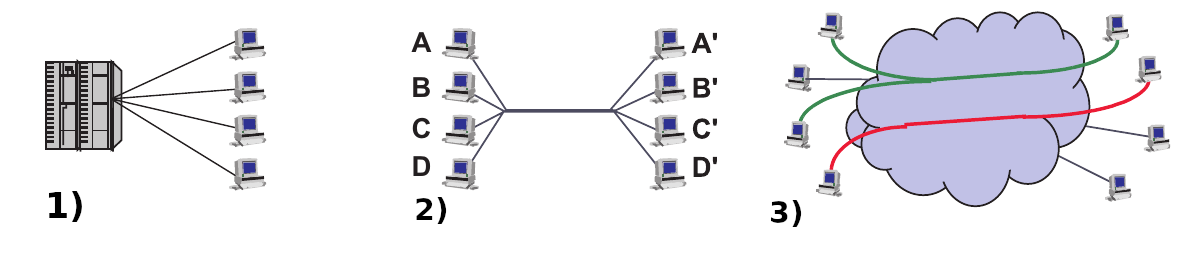
\includegraphics[scale=0.4]{images/3-2.png} 
     	%\vspace*{-0.5em}
		%\caption{Floating gate transistor cell}
	\end{figure}	
	\end{center}	
		
	\end{frame} 
	
	\subsection{Concentrators}

	\begin{frame}

	\begin{center}	
	\begin{figure}
		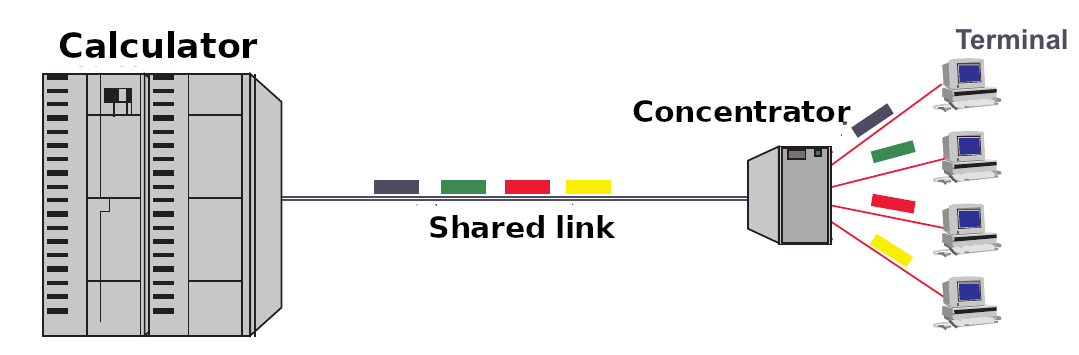
\includegraphics[scale=0.35]{images/3-3.png} 
     	%\vspace*{-0.5em}
		%\caption{Floating gate transistor cell}
	\end{figure}	
	\end{center}	
			
	The concentrator analyses the content of the blocks of data and redirect the data to the right terminal. Terminals can send back information to the concentrator as well. 

	\begin{block}{Notes}
	\begin{itemize}
	\item{Note that concentrators are a little bit outdated. A "gateway" computer can be used instead to reproduce the same behavior of a concentrator.}
	\item{Here a terminal cannot communicate with another one!}
	\item{Concentrators look like hubs or switches but actually there are different: concentrators allow a static 1 -> N configuration (with a hub or a switch the origin can be different each time).}
	\end{itemize}
	\end{block}
	
	\end{frame}
	
	\subsection{Multiplexers}
	
	\begin{frame}
	
	A multiplexer is a device putting in relation one user from one side to another using a shared connection line.	
	\vspace*{1em}
	
	\begin{center}	
	\begin{figure}
		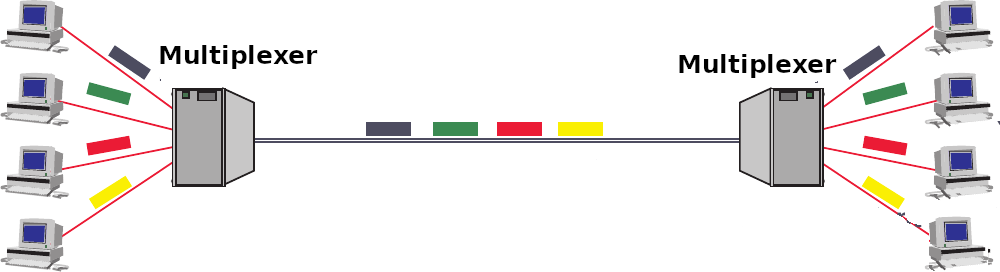
\includegraphics[scale=0.4]{images/3-4.png} 
     	%\vspace*{-0.5em}
		%\caption{Floating gate transistor cell}
	\end{figure}	
	\end{center}		
	\vspace*{1em}
	
	Grouping all the blocks together on one line is called: multiplexing.	
	
	\end{frame}	
	
	\subsection{Networks}	
	
	\begin{frame}
	
	Multiplexers and concentrators are limited. Only networks ensure an open connectivity (1->1 to N or even M-> 1 to N).	
	\vspace*{1em}	

	\begin{block}{Definition}
	A network is a set of hardware and software geographically spread to ensure data transportation in an open connectivity way.
	\end{block}
	\vspace*{1em}

	\begin{center}	
	\begin{figure}
		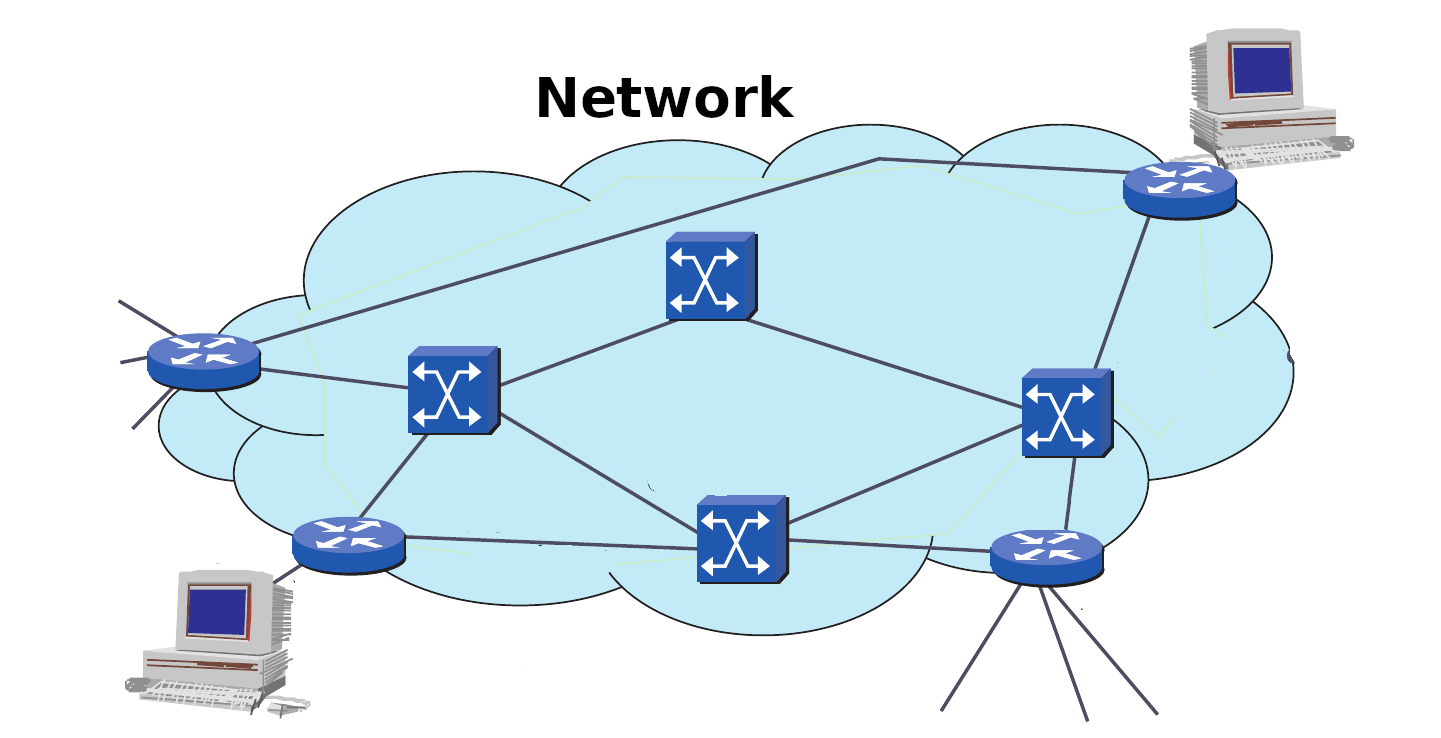
\includegraphics[scale=0.35]{images/3-5.png} 
     	%\vspace*{-0.5em}
		%\caption{Floating gate transistor cell}
	\end{figure}	
	\end{center}		
	
		
	\end{frame}	
	
	\begin{frame}
	
	There are three classes of network:
	\vspace*{1em}
	
	\begin{itemize}
	\item{LAN (Local Area Network): a local network restricted to small area (ex: a building, a room, etc...). Usually the bandwidth is high in that case: 10 to 100Mbit/s.}
	\item{MAN (Metropolitain Area Network): this network can be geographically expanded up to 100km long. This network is generally used to gather the local networks and ensure a communication between them (ex: university network).}
	\item{WAN (Wide Area Network): these networks generally ensure information over a very large distance (require a subscription to access this network, and is generally slower then LAN.}
	\end{itemize}		
		
	\end{frame}	
	
	\subsection{Physical topography of networks}	
	
	\begin{frame}
	
	The topography of a network defines how the computers (or nodes) are connected each other.
	\vspace*{1em}
	
	Elementary ways to link nodes:	
	
	\begin{center}	
	\begin{figure}
		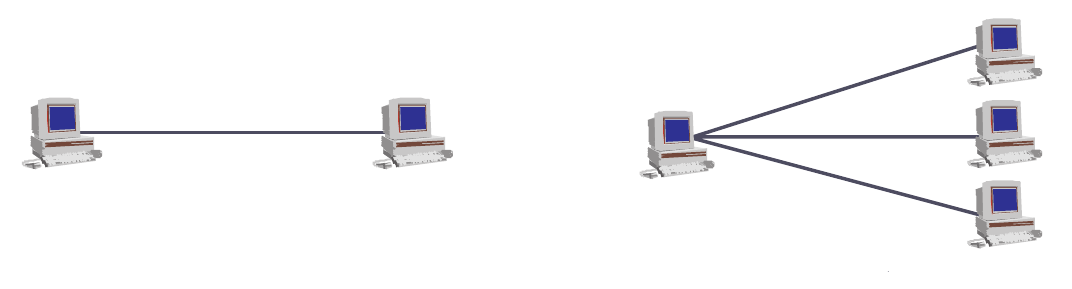
\includegraphics[scale=0.55]{images/3-6.png} 
     	%\vspace*{-0.5em}
		%\caption{Floating gate transistor cell}
	\end{figure}	
	\end{center}	
	
	Point-to-point	(left) and 	Multi-points (right)
	
	\end{frame}	
	
	\begin{frame}
	
	Basic topographies:
	
	\begin{center}	
	\begin{figure}
		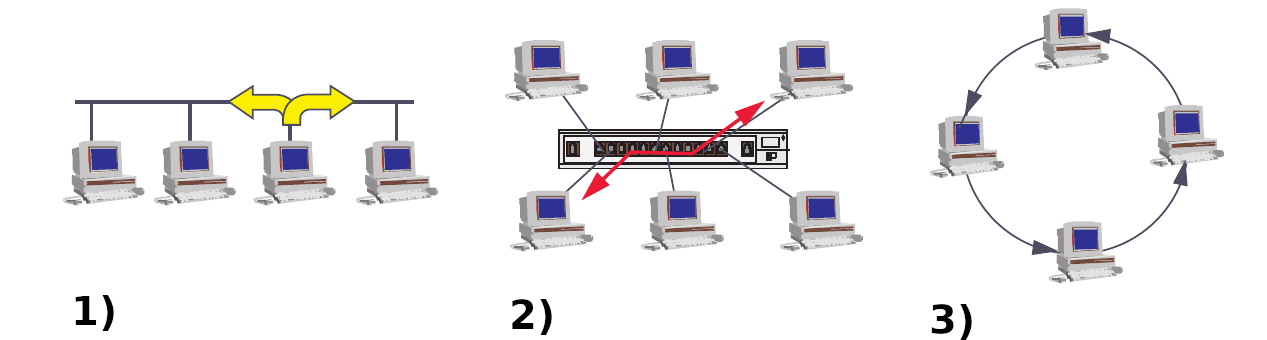
\includegraphics[scale=0.55]{images/3-7.png} 
     	%\vspace*{-0.5em}
		%\caption{Floating gate transistor cell}
	\end{figure}	
	\end{center}
	
	Bus	(1), Star (2) and Ring (3).
	
	\end{frame}	
	
	\begin{frame}

	\begin{itemize}
	\item{Bus: Information is emitted over all the network. It can suffer from collisions (require an access policy (like polling/send). This kind of architecture is cheap and it's easy to add a new computer (while not disturbing the current communication).}
	\item{Star: All the nodes are connected to a central node. More complex, but allow fast inter-node communications. If one node is failling, this does not impact the network. Still the network relies on a central node.}
	\item{Ring: Each node is connected to the next. Information moves in one direction only. Each node receives the data and regenerate it (if the data is arrived in the right node: data is copied and processed).}
	\end{itemize}
	
	\end{frame}	
	
	\begin{frame}
	
	Built topographies:
	\vspace*{1em}
	
	More complex topographies can be built by combining "star" and "bus" topographies together, for instance.
	\vspace*{0.5em}
	
	We can build for instance hierarchical topographies (1 and 2) or mesh topographies (3).
	\vspace*{1em}
	
	\begin{center}	
	\begin{figure}
		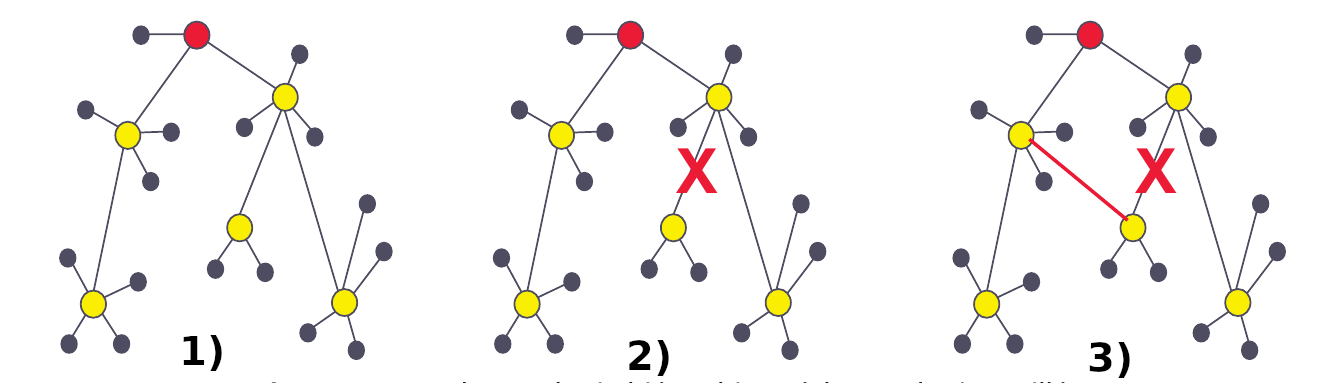
\includegraphics[scale=0.5]{images/3-8.png} 
     	%\vspace*{-0.5em}
		%\caption{Floating gate transistor cell}
	\end{figure}	
	\end{center}
	

	\begin{block}{Note}A mesh topography is more robust!\end{block}
	
	\end{frame}	
	
	\begin{frame}
	
	Let's imagine we want to connect 4 computers with a 1->1 to N relation (network concentration).
	\vspace*{1em}
	
	\begin{center}	
	\begin{figure}
		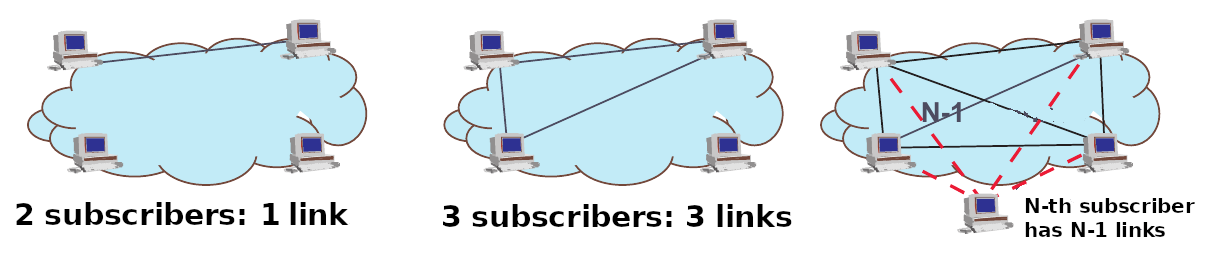
\includegraphics[scale=0.55]{images/3-9.png} 
     	%\vspace*{-0.5em}
		%\caption{Floating gate transistor cell}
	\end{figure}	
	\end{center}
	
	In this case we need 6 links!
	\vspace*{1em}
	
	$Number\ of\ links = \frac{N(N-1)}{2}$
	\vspace*{0.5em}
	
	Now let's imagine we are dealing with $300\times 10^6$ internet subscribers (now there are more subscribers worldwide).	
	\vspace*{1em}
	
	We would need in that case: $45\times 10^{15}$ links!!! Obviously this number enormous! 
		
	\end{frame}	
	
	
	\begin{frame}
	
	This just demonstrates the necessity to handle connections differently... This is the switching network.	
	\vspace*{1em}
	
	Now we can have this:
	\vspace*{1em}
	
	\begin{center}	
	\begin{figure}
		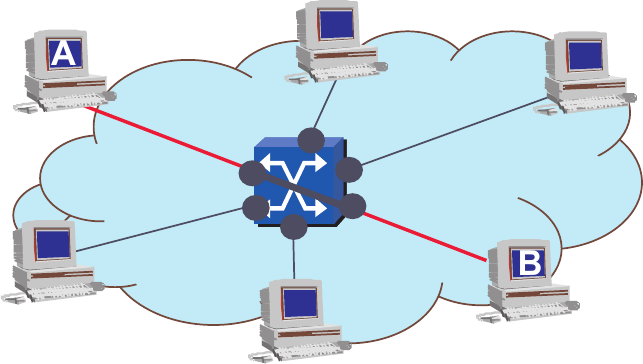
\includegraphics[scale=0.5]{images/3-10.png} 
     	%\vspace*{-0.5em}
		%\caption{Floating gate transistor cell}
	\end{figure}	
	\end{center}
	\vspace*{1em}
	
	Ex: the switch put in relation A and B, so they can exchange data.
	
	\end{frame}		
	
	\section{Switched networks}	
	
	\begin{frame}
	
	Now we can distinguish two different views of the same network:
	\vspace*{1em}
	
	\begin{center}	
	\begin{figure}
		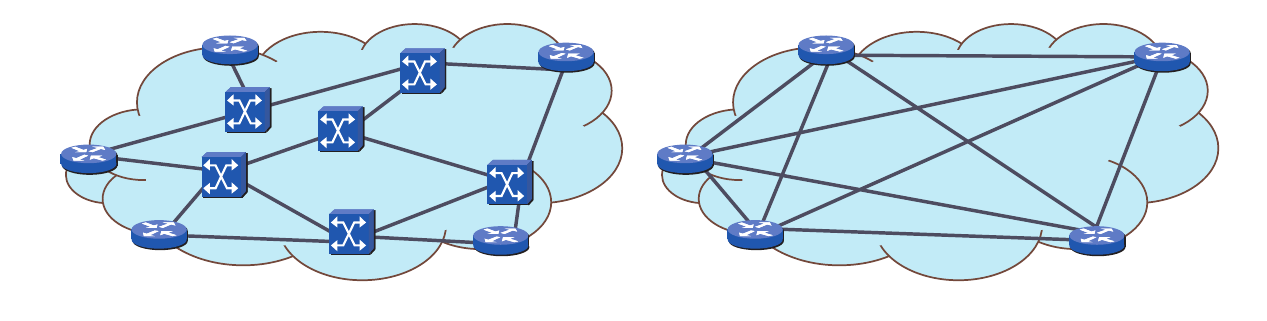
\includegraphics[scale=0.55]{images/3-11.png} 
     	%\vspace*{-0.5em}
		%\caption{Floating gate transistor cell}
	\end{figure}	
	\end{center}
	
	Physical view (left) and logical view (right).	
	\vspace*{0.5em}
	
	Three switch network approaches:
	\vspace*{1em}
	
	\begin{itemize}
	\item{Circuit-switched network}
	\item{Message-switched network}
	\item{Packet-switched network}
	\end{itemize}
		
	
	\end{frame}	
	
	\subsection{Circuit-switched network}	
	
	\begin{frame}
	
	Circuit switched network:
	\vspace*{0.5em}
	
	With this kind of switching approach: a physical link is established between the source and the destination (point-to-point connection).
	\vspace*{0.5em}
	
	This physical point-to-point connection is realized by the switch(es) before exchanging data, and this connection is maintained during all the communication.
	\vspace*{0.5em}
	
	The rate of connections can be very high whereas the rate of activity can be low (each physical connection is only used for one exchange: not optimized)  

	\begin{center}	
	\begin{figure}
		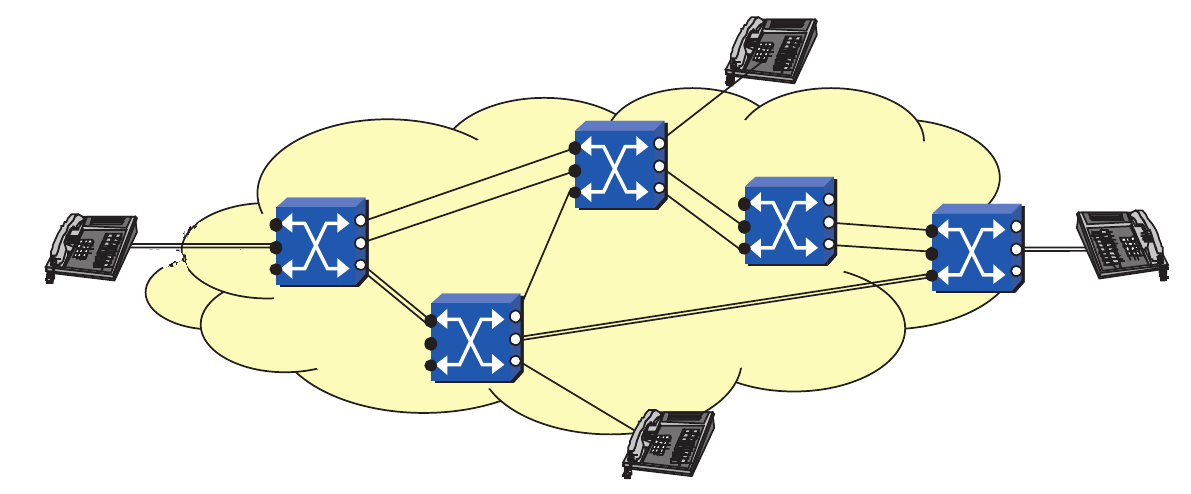
\includegraphics[scale=0.3]{images/3-12.png} 
     	%\vspace*{-0.5em}
		%\caption{Floating gate transistor cell}
	\end{figure}	
	\end{center}
	
	Circuit-switched network of old-fashion phone network.

	\end{frame}

	\subsection{Message-switched network}

	\begin{frame}
	
	Message-switched network:
	\vspace*{0.5em} 
	
	With message-switched network no physical connections is established. Instead messages are sent node to node (and wait in intermediary nodes if the link is currently occupied). Each message is a block of information (piece of a file, etc...). The data to transmit is divided into messages. Messages are stored in each node and send in the rest of the network (if the link is free).
	\vspace*{0.5em}
	
		\begin{center}	
	\begin{figure}
		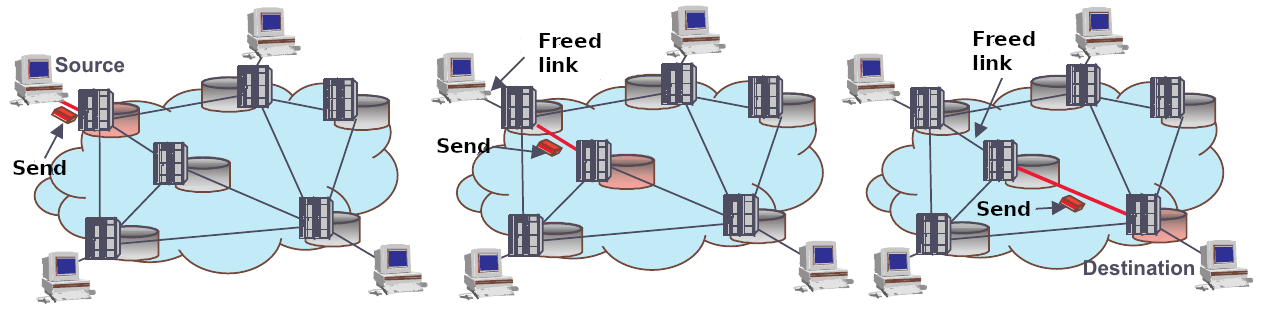
\includegraphics[scale=0.45]{images/3-13.png} 
     	%\vspace*{-0.5em}
		%\caption{Floating gate transistor cell}
	\end{figure}	
	\end{center}	
	
	This approach is more optimized. Still, this approach is not suited for interactive applications (For very important applications: MMORPG, FPS, etc...). 
	
	\end{frame}

	\subsection{Packet-switching network}

	\begin{frame}
	
	Packet-switching network:
	\vspace*{0.5em}
	
	This is the modern switching approach.
	
	Like for the message-switched network the data to be transmitted is subdivided in fragments: here called "packets". 
	
	But: contrary to the message-switch networks: intermediary nodes don't store the packets, but send them on-the-fly (send them immediately). Each node receiving a packet send it back immediately using the route that is optimal at the moment (nodes don't used much memory). Packets from different sources can be handled by a same node.     
		
	\begin{center}	
	\begin{figure}
		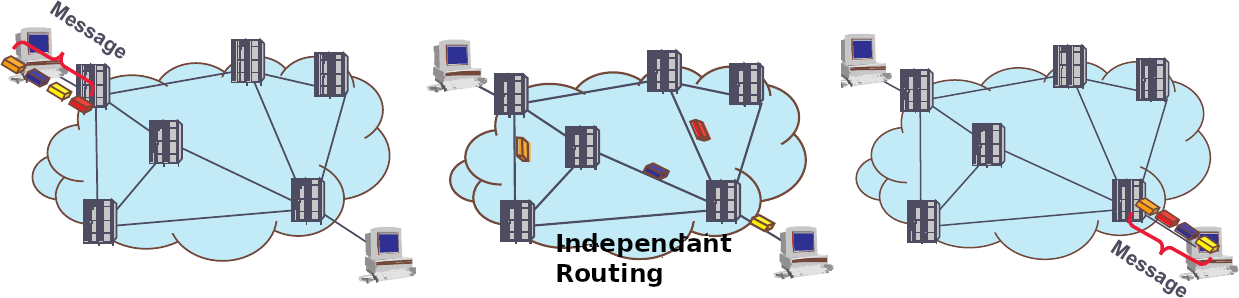
\includegraphics[scale=0.5]{images/3-14.png} 
     	%\vspace*{-0.5em}
		%\caption{Floating gate transistor cell}
	\end{figure}	
	\end{center}
	
	With this approach packets can arrive at destination in different orders: so in each packet we must have information to rebuild the data at the end.	
	
	\end{frame}
		
	\subsection{Circuit-switched or packet-switched network}		
		
	\begin{frame}
	
	Circuit-switched or packet-switched network:
	\vspace*{1em}
	
	Packet-switched network: for each packet, the optimal route is seeked (sending packets in order is not guaranteed).
	\vspace*{1em}
	
	This kind of network is also called "best-effort".
	\vspace*{1em}
	
	Circuit-switched network: data is sent sequentially (one physical link is established and is used until the end).   	
	\vspace*{1em}

	\begin{block}{But could we mix the advantages of both approaches?}
	This would ensure the sequencing of the data while optimizing how the network is used: this is the connection-oriented mode.
	\end{block}
	
	\end{frame}
		
	\subsection{Connection-oriented mode}		
		
	\begin{frame}
	
	With this approach a virtual circuit is established before the data transmission between the source and the receptor. 
	\vspace*{1em}
	
	This circuit can be permanent (PVC: Permanent Virtual Circuit) or established when needed (SVC: Switched Virtual Circuit).
	\vspace*{0.5em}
	
	\begin{center}	
	\begin{figure}
		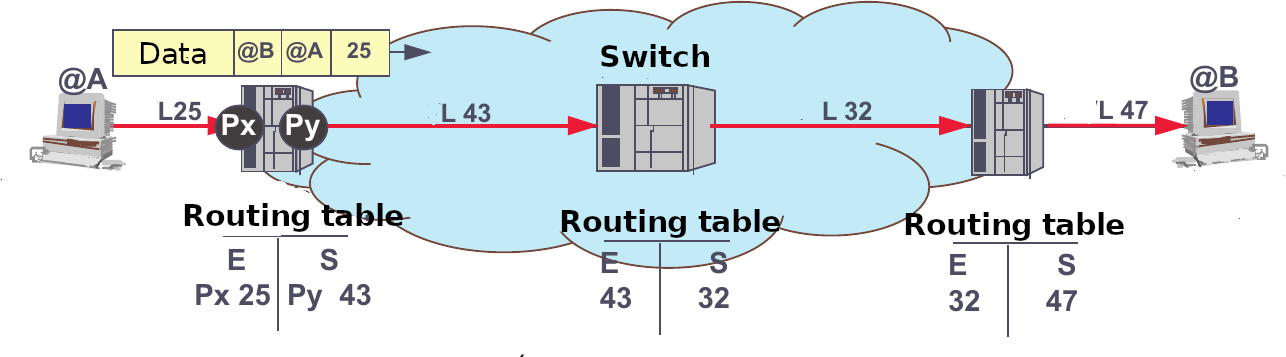
\includegraphics[scale=0.5]{images/3-15.png} 
     	%\vspace*{-0.5em}
		%\caption{Floating gate transistor cell}
	\end{figure}	
	\end{center}
	
	So here the virtual circuit simply follows: L25, L43, L32 and L47.
	
	\end{frame}

	\begin{frame}
	
	Connection-oriented or connection-less mode?	
	\vspace*{1em}
	
	The mode of connection is defined by the protocol used for the communication. Choosing a connection-oriented or connection-less mode depends on the performances and the quality of service we want.
	\vspace*{0.5em}
	
	Permanent Virtual Circuit or Switched Virtual Circuit?
	\vspace*{1em}
	
	All the connection-oriented protocols offer two possibilities but: SVC still requires too much computation to work for very large networks (WAN). For WAN: PVC is preferred (routing tables are "manually" defined). Defining a routing table can be done using a communication matrix.
	
	\begin{center}	
	\begin{figure}
		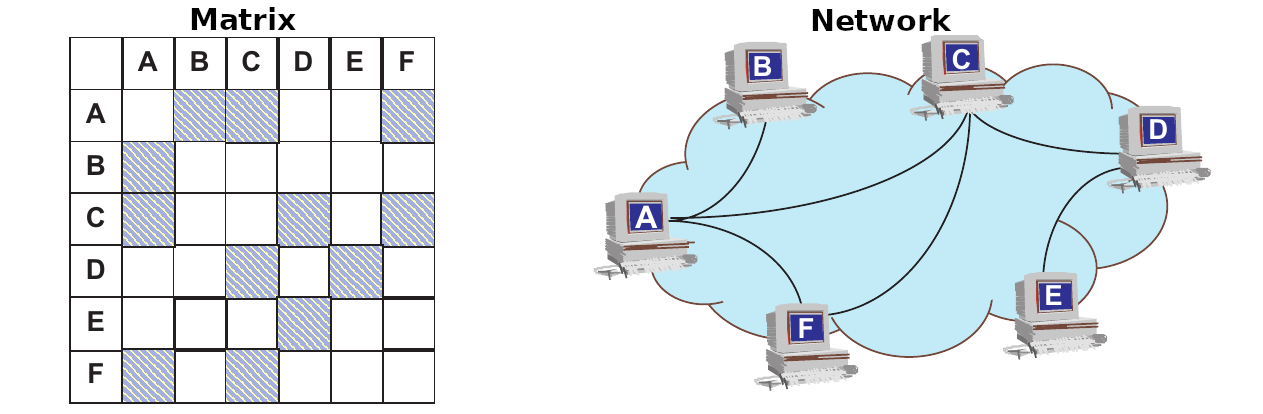
\includegraphics[scale=0.35]{images/3-16.png} 
     	%\vspace*{-0.5em}
		%\caption{Floating gate transistor cell}
	\end{figure}	
	\end{center}
	
		
	\end{frame}

	\subsection{Addresses}
	
	\begin{frame}
	
	When sending its message the source must provide an address to identify/reach the destination.
	\vspace*{1em}
	
	An address is a sequence of characters identifying a physical point of connection in a network (physical address) or, identifying a process/a computer (logical address). These two notions are complementary: one defines the object (physical address) the other defines its localization (logical address).
	\vspace*{1em}
	
	We will talk about logical addresses later. To locate a computer in the network you need to know: 
	\vspace*{1em}
	
	\begin{itemize}
	\item{The network on which it is connected}
	\item{The access point attached to the network}
	\item{The target computer}
	\end{itemize}	  
	
	
	\end{frame}

	\begin{frame}
	
	\begin{center}	
	\begin{figure}
		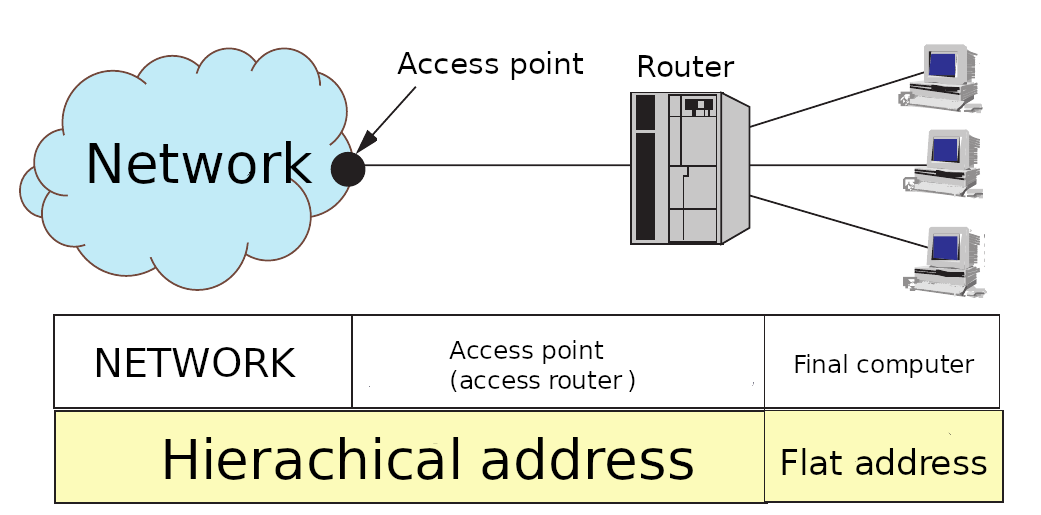
\includegraphics[scale=0.4]{images/3-17.png} 
     	%\vspace*{-0.5em}
		%\caption{Floating gate transistor cell}
	\end{figure}	
	\end{center}
	\vspace*{1em}
	
	The first two fields are used to locate the local installation. The last field is used to identify the destination within the final installation. 
	\vspace*{1em}
	
	\begin{block}{Note}
	We will not talk about hierarchical addressing in this course, since we will talk about IP addresses in the next course.
	\end{block}
		
	\end{frame}
	
	\begin{frame}
	
	The flat address is called MAC (Medium Access Control) and is organized as follows:
	\vspace*{1em}
	
	\begin{center}	
	\begin{figure}
		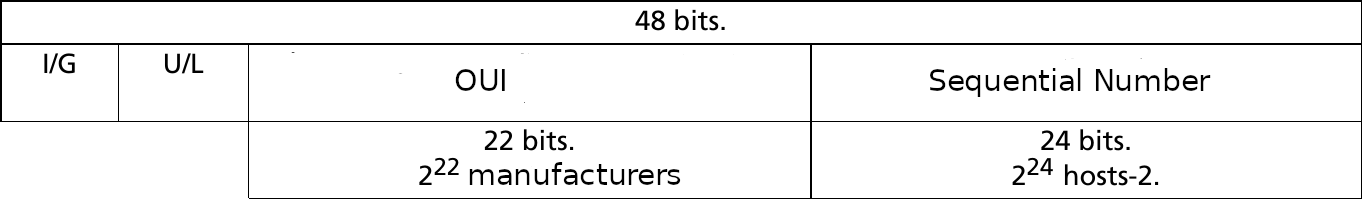
\includegraphics[scale=0.4]{images/3-18.png} 
     	%\vspace*{-0.5em}
		%\caption{Floating gate transistor cell}
	\end{figure}	
	\end{center}
	
	OUI (Organizational Unit Identifier) identify the manufacturer of the network card of the computer (you can consider it identify the manufacturer of the computer itself if you want, although not always the case).
	\vspace*{1em}

	The sequential number is given buy the manufacturer, and ensure the uniqueness of the MAC address worldwide.	
		
	\end{frame}	
	
	\section{Routing the network}
	
	\subsection{What is it?}
	\begin{frame}
	
	Routing information through the network consists in permitting the transmission of data from a certain entry point to an exit point designed by an address.
	\vspace*{1em}
	
	Each node of the network has a routing table.
	\vspace*{0.5em}	
	
	A routing table is made of triplets: destination address, route to follow and cost.
	\vspace*{0.5em}	
	
	\begin{center}	
	\begin{figure}
		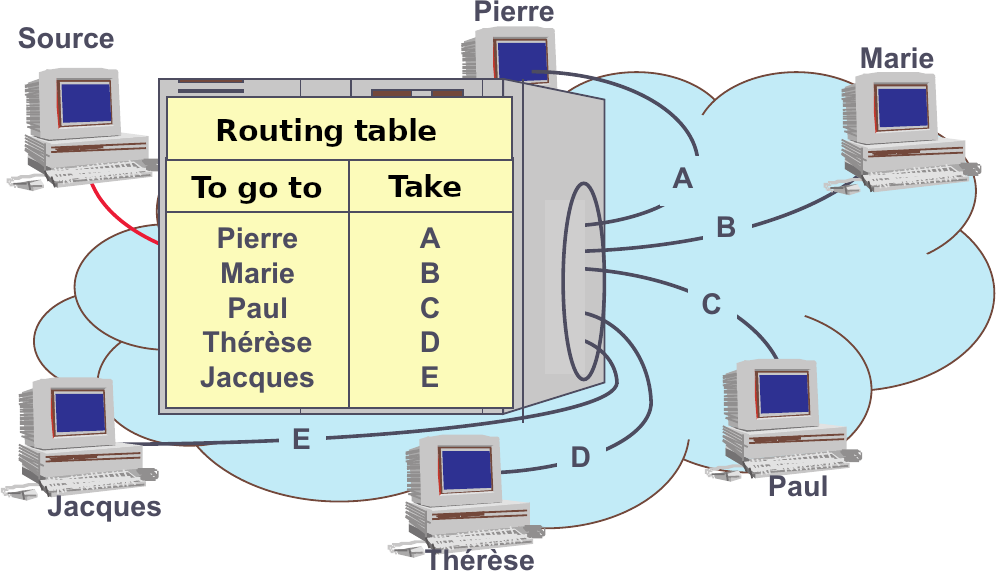
\includegraphics[scale=0.4]{images/3-19.png} 
     	%\vspace*{-0.5em}
		%\caption{Floating gate transistor cell}
	\end{figure}	
	\end{center}
		
	\end{frame}

	\subsection{Routing policies and modes}

	\begin{frame}
	
	There are three routing policies:
	\vspace*{1em}
	
	\begin{itemize}

	\item{Deterministic: the routing tables are static (the routing will not change from one point A to one point B).}
	\item{Adaptive: each node adapts its routing table based on its knowledge of the state of the networks.}
	\item{Mixed: adaptive for establishing the route and deterministic after (for further usages).}	
	
	\end{itemize}		
	
	\end{frame}
	
	\begin{frame}
	
	Different routing modes:
	\vspace*{0.5em}
	
	\begin{enumerate}
	\item{Static routing: for each node a routing table is built by a system administrator (to go from A to B). This approach is simple but no solution if node B crashes (A->B->C).}
	\item{Broadcast routing: information is sent to several nodes (N nodes). Each of these nodes send to N other nodes until destination.}
	\item{Flood routing: the node send information all all its output lines (except the line sending the initial message) until destination. This is very robust but can overload the network (used by military). We are guarantee to find the shortest path each time.}
	\item{Lowest cost routing: here each node has a routing table giving the next path in order to ensure the lowest cost routing. This path is followed to transmit the message.}	
	\end{enumerate}			
	
	
	\end{frame}
	
	\begin{frame}	
	
	The lowest-cost routing is based on a cost:
	\vspace*{0.5em}
	
	\begin{itemize}
	\item{meters}
	\item{latency time}
	\item{reliability}
	\item{...}	
	\end{itemize}		
	\vspace*{1em}		
		
	There are different ways to ensure a lowest-cost routing:
	\vspace*{0.5em}
	
	\begin{enumerate}
	\item{Distance vector routing (Bellman-Ford): iteratively learn the best route.}
	\item{Link-state routing (Dijkstra algorithm, based on binary trees): computing best route based on link states.}		
	\end{enumerate}			
		
	\end{frame}
	
	\begin{frame}
	
	Distance vector routing:
	
		\begin{center}	
	\begin{figure}
		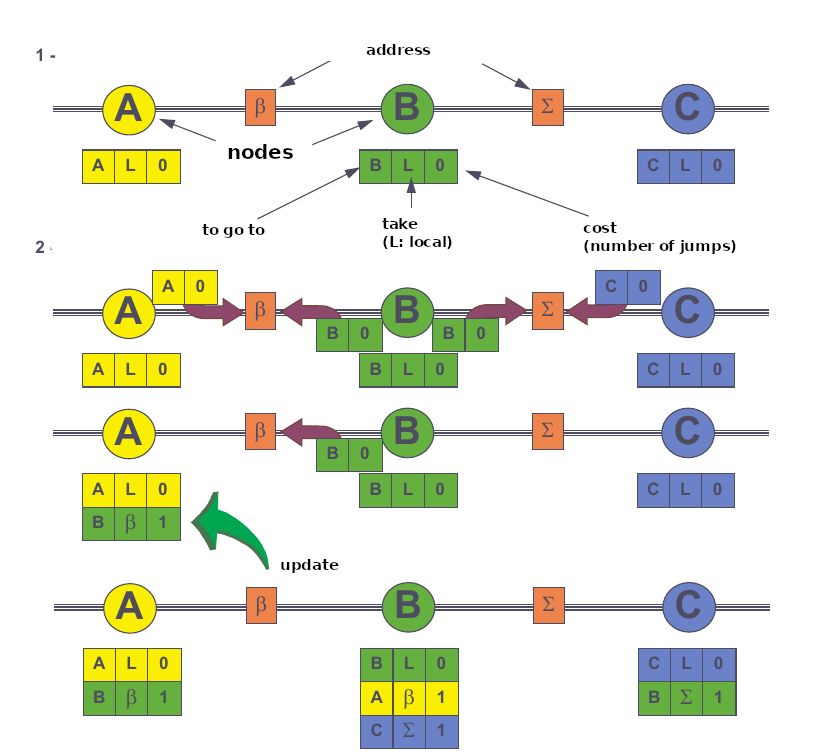
\includegraphics[scale=0.45]{images/3-20.png} 
     	%\vspace*{-0.5em}
		%\caption{Floating gate transistor cell}
	\end{figure}	
	\end{center}
	
	
	\end{frame}
	
	\begin{frame}
	
		\begin{center}	
	\begin{figure}
		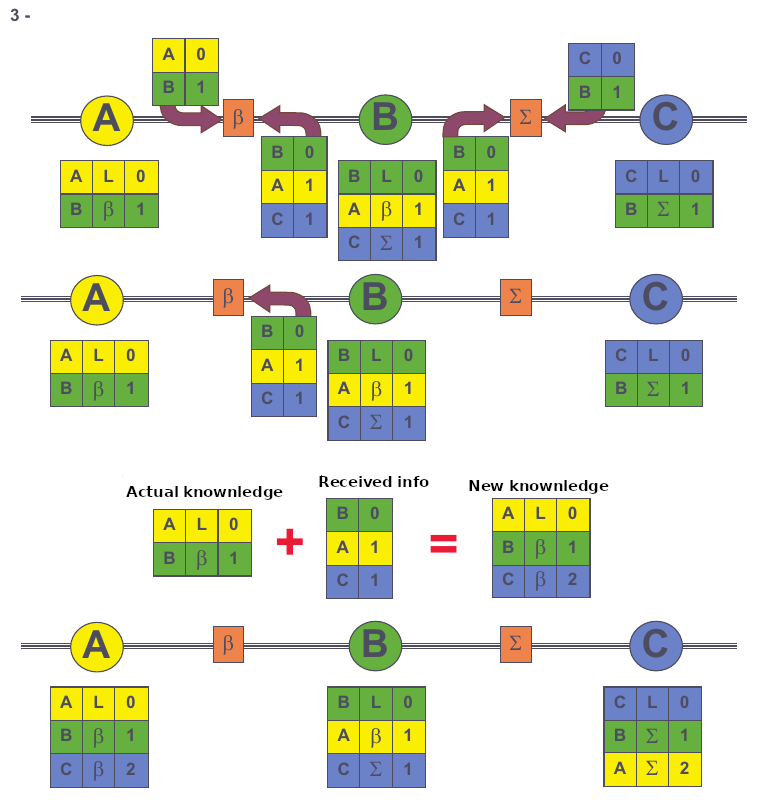
\includegraphics[scale=0.4]{images/3-21.png} 
     	%\vspace*{-0.5em}
		%\caption{Floating gate transistor cell}
	\end{figure}	
	\end{center}
		
	Distance vector routing is the most used approach. But there are two main drawbacks:
		
	\begin{itemize}
	\item{Table convergence is slow}
	\item{Loops can be created in the network}	
	\end{itemize}		
	
	\end{frame}	
	
	\begin{frame}
	
	Link-state routing:
	\vspace*{1em}
	
	In this case each node determine the cost for each link:
	\vspace*{0.5em}
	
	\begin{itemize}
	\item{In case of modification, this information is sent through the network: the triplet (A, B, c) is sent. A is the origin node, B the destination node and c the cost to go from A to B.}
	\item{Each node has a matrix of cost.}
	\item{The table of routing is built using an algorithm (Dijkstra, ...)}
	\end{itemize}	
	
	\end{frame}	
	
	\begin{frame}
	
	For both approaches specific protocol are used: routing protocols.
	\vspace*{1em}
	
	These protocols ensure the building and the updating of the routing tables of the network.
	\vspace*{0.5em}
	
	Two examples of routing protocols:
	\vspace*{0.5em}
	
	\begin{itemize}
	\item{RIP: Routing Information Protocol}
	\item{OSDF: Open Shortest Path First}
	\item{...}
	\end{itemize}		
	
	\end{frame}
	
	\section{MTU}
	
	\begin{frame}
	
	When a block of data is send in the network each node/switch must save, process and release the block of data.	
	\vspace*{0.5em}
	
	But resources are limited!
	\vspace*{0.5em}
	
	A switch can process only a restricted number of blocks ...
	\vspace*{0.5em}
	
	
		\begin{center}	
	\begin{figure}
		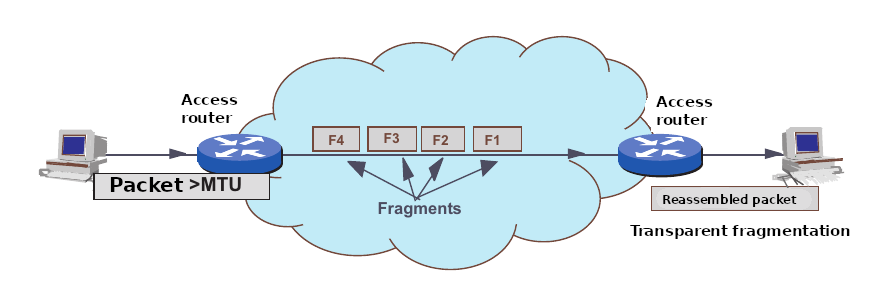
\includegraphics[scale=0.4]{images/3-22.png} 
     	%\vspace*{-0.5em}
		%\caption{Floating gate transistor cell}
	\end{figure}	
	\end{center}
	
	MTU is the maximum traffic unit. This is the maximal size a block can have in the network. 	
	\vspace*{0.5em}
	
	If a packet has a size bigger than MTU, the packet needs to be split.	
	
	\end{frame}
	
	
	
	



\end{document}